\documentclass[12pt]{article}
\usepackage{geometry} 
\geometry{letterpaper}
\usepackage{graphicx}
\usepackage{Sweave}

% \VignetteIndexEntry{How to use the ss3sim package to run simulations in SS3}
% \VignetteKeyword{metapopulations}
% \VignetteKeyword{ecology}

%\usepackage[round]{natbib} 
%\bibliographystyle{apalike}   
%\bibpunct{(}{)}{;}{a}{}{;}   

\title{How to use the \texttt{ss3sim} package to run\\simulations in SS3}
\author{Sean C. Anderson, \ldots}
\date{}

\begin{document}
\maketitle

\noindent
First start by installing the latest version of \texttt{ss3sim} and loading the 
package:

\begin{Schunk}
\begin{Sinput}
> # install.packages("devtools")
> # devtools::install_github("ss3sim", username="seananderson")
> library(ss3sim)
\end{Sinput}
\end{Schunk}

\noindent
You can read the help files and access this vignette again with:

\begin{Schunk}
\begin{Sinput}
> help(package = "ss3sim")
> vignette("ss3sim")
\end{Sinput}
\end{Schunk}

\section*{Setting up the file structure}
This package is set up assuming that you have an established base case 
operating model and estimation model to work with. Each operating model and 
estimation model should be in their own folder. The operating should have the 
files:
\begin{enumerate}
  \item \texttt{yourmodel.ctl}
  \item \texttt{yourmodel.dat}
  \item \texttt{ss3.par}
  \item \texttt{starter.ss}
\end{enumerate}

The estimation model folder should have:

\begin{enumerate}
  \item \texttt{yourmodel.ctl}
  \item \texttt{yourmodel.dat}
  \item \texttt{starter.ss}
\end{enumerate}

In both cases, nothing more and nothing less. The names of the \texttt{.ctl} 
and \texttt{.dat} files are not important. The package functions will rename 
them after they are copied to appropriate folders. These files should be 
derived from the \texttt{.ss\_new} files but named as listed above. It's 
important to use these \texttt{.ss\_new} files so they have consistent 
formatting. Many of the functions in this package depend on that formatting.

For the purposes of the Fish 600 project, we have unique case identifiers which 
combine to create unique scenarios. The types of cases are: natural mortality 
(M), fishing mortality (F), data quality (D), and retrospective (R). And the 
species are cod (cod), sardine-like (sar), and flatfish (fla). It's important 
to use these three letter abbreviations for the species since the functions 
assume that the last three letters represent a species (or some other 
identifier for a different project).

The different version of each case are identified with numbers. So, for 
example, the base case scenario for cod is identified as 
\texttt{M1-F1-D1-R1-cod}. We will have a spreadsheet that describes each of 
these in plain language.

%For example, for a scenario might have these folders:

%\begin{verbatim}
%M1F1D1R1-cod
%M1F1D1R1-fla
%M1F1D1R1-sar
%\end{verbatim}


%Once you have these folders set up you can move them into the simulation folder 
%structure with the \texttt{copy\_ss3model} function. Assuming you've put these 
%in folders called \texttt{operating-models} and \texttt{estimation-models} you 
%can copy the models over like this:

%<<eval = FALSE, echo = true>>=
%copy_ss3models(model_dir = "operating-models", type = "om")
%copy_ss3models(model_dir = "estimation-models", type = "em")
%@

%\noindent
%or if you were only responsible for 1:50:

%<<eval = FALSE, echo = true>>=
%copy_ss3models(model_dir = "operating-models", type = "om", 
  %iterations = 1:50)
%@

The function \texttt{copy\_ss3models} creates a folder structure and copies 
over the operating and estimation models. The folder structure looks like:

\begin{verbatim}
  M1-F1-D1-R1-cod/1/om
  M1-F1-D1-R1-cod/1/em
  M1-F1-D1-R1-cod/2/om
  M1-F1-D1-R1-cod/2/em
  ...
\end{verbatim}

If you are using bias correction (\texttt{bias\_correct = TRUE}) then there 
will be some additional folders. In that case the folders will look like:

\begin{verbatim}
  M1-F1-D1-R1-cod/bias/1/om
  M1-F1-D1-R1-cod/bias/1/em
  M1-F1-D1-R1-cod/bias/2/om
  M1-F1-D1-R1-cod/bias/2/em
  ...
  M1-F1-D1-R1-cod/1/om
  M1-F1-D1-R1-cod/1/em
  M1-F1-D1-R1-cod/2/om
  M1-F1-D1-R1-cod/2/em
  ...
\end{verbatim}

\noindent
Note that the operating and estimating model folders have been renamed
\texttt{om} and \texttt{em} within each iteration, the operating and estimation 
models have been checked to make sure they contain the minimal files (as listed 
above), the filenames have been made all lowercase, the data file has been 
renamed \texttt{data.dat}, the control files have been renamed \texttt{om.ctl} 
or \texttt{em.ctl}, and the starter and control files have been adjusted to 
reflect these new file names.

The functions in this package assume you've set your working directory in R to 
be the base folder where you will store the scenario folders.

\section*{Creating the input configuration files}
You will need to have a folder containing ``case'' argument definitions. These 
plain text files are read by \texttt{get\_caseval} and turned into argument 
lists that are passed to \texttt{run\_ss3sim}. You can create template input 
files by running \texttt{create\_argiles}. It reads the various functions and 
parses the arguments and default values into plain text files. The default 
settings create these files:

\begin{enumerate}
  \item \texttt{M0-spp.txt}
  \item \texttt{F0-spp.txt}
  \item \texttt{index0-spp.txt}
  \item \texttt{agecomp0-spp.txt}
  \item \texttt{lcomp0-spp.txt}
  \item \texttt{R0-spp.txt} (not implemented yet)
\end{enumerate}

Look in your working directory for the template files. Change the case ID 
number (defaults to \texttt{0}) and the species identifier to a three letter 
identifier. For the Fish 600 project use one of \texttt{cod}, \texttt{sar}, or 
\texttt{fla} for cod, sardine, or flatfish. An example filename would be 
\texttt{M1-sar.txt} or \texttt{lcomp2-fla.txt}.

The first column in the text files denotes the argument to be passed to a 
function. The second argument denotes the value to be passed. You can use any 
simple R syntax. For example: \texttt{c(1, 2, 4)}, or \texttt{seq(1, 100)} or 
\texttt{1:100} or \texttt{matrix()}. Character objects don't need to be quoted, 
but can be if you'd like. However, be careful not to use the delimiter (set up 
as a semicolon) anywhere else in the file besides to denote columns. You can 
add comments after any \texttt{\#} symbols. Internally, the functions evaluate 
in R any entries that have no character values (e.g. \texttt{1:100}) or have an 
alpha-numeric character followed by a \texttt{(}. Anything that is character 
only or has character mixed with numeric but doesn't have the regular 
expression \texttt{"[A-Za-z0-9]("} gets turned into a character argument.

Putting that all together, here's what an example \texttt{F1-cod.txt} file 
might look like:

\begin{verbatim}
years; 1:100
years_alter; NA 
fvals; NA
\end{verbatim}

\section*{Running the models}

The \texttt{run\_ss3sim} function is a wrapper function. It adjusts the natural 
mortality, adjusts the fishing mortality, adds recruitment deviations, calls 
\texttt{run\_ss3model} to run the operating model, samples various survey 
estimates from the operating model, changes the age composition data as 
specified, changes the length composition data as specified, copies and renames 
files as necessary, and calls \texttt{run\_ss3model} again to run the 
estimation model.

The \texttt{run\_fish600} function is a high-level wrapper that deals with 
parsing the case input files and then passes these arguments on to 
\texttt{run\_ss3sim}.

Say you have your input case files setup and you want to run the first 
50 iterations of those scenarios. You could run them like this:

\begin{Schunk}
\begin{Sinput}
> # First grab the example package data:
> d <- system.file("extdata", package = "ss3sim")
> f <- paste0(d, "/run_ss3sim_eg/")
> om_model_dir <- paste0(f, "cod_om")
> em_model_dir <- paste0(f, "cod_em")
> case_folder <- paste0(f, "case-arguments")
> #
> #
> # Without bias correction:
> run_fish600(iterations = 1, scenarios = c("M1-F1-D1-R1-cod"),
+ case_folder = case_folder, om_model_dir = om_model_dir,
+ em_model_dir = em_model_dir)
> #
> #
> # With bias correction:
> # (Note that bias_nsim should be bigger, say 5, but it is set to 1
> # here so the example runs faster.)
> run_fish600(iterations = 1, scenarios = c("M1-F1-D1-R1-cod"),
+ case_folder = case_folder, om_model_dir = om_model_dir,
+ em_model_dir = em_model_dir, bias_correct = TRUE,
+ bias_nsim = 1)
\end{Sinput}
\end{Schunk}


\section*{The flat scenario ID structure}
There are many advantages to this flat scenario ID fold setup:

\begin{enumerate}
  \item It makes it easier for multiple papers to share scenarios.

  \item It makes it easier for papers to change which scenarios to compare 
    after.

  \item It avoids unnecessary nested folder structure.

  \item It's easier to distribute the model runs across people and computers.

  \item The functions are more general and applicable to future research.

  \item Since each folder represents a unique scenario run, it's simple to keep 
    track of progress on model runs in a spreadsheet
  
\end{enumerate}

\noindent
We can have a spreadsheet with the following columns:

\begin{verbatim}
Scenario ID, Scenario description, Model status
\end{verbatim}

\noindent
Then, groups can compile a list of scenario IDs they want to extract and 
compare.



%\section*{Setting up the models}

%The main functions to work with are:

%\begin{description}
  %\item[\texttt{change\_f}] A function to alter fishing mortality values in the \texttt{.par} file

  %\item[\texttt{change\_m}] Adds time-varying natural mortality either through the environment, block, or deviation methods.
%\end{description}

%ADD EXAMPLES OF USING THESE FUNCTIONS FOR COMMON SCENARIOS

%\section*{What \texttt{run\_ss3sim} does}

%Between running the operating and estimation models, \texttt{run\_scenario} performs a number of tasks that are needed across all scenarios:

%\begin{enumerate}
  %\item Takes the appropriate column of recruitment deviations from \texttt{data(recdevs)}, scales them by the appropriate standard deviation using \texttt{TODO}, and adds them to the \texttt{.par} file using \texttt{change\_rec\_devs}. \item Samples the length and age composition data and adds them to the data file using \texttt{change\_lcomp} and \texttt{change\_agecomp}.
  %\item Jitters the index of abundance based on the reported biomass for each fleet using \texttt{jitter\_index}.
  %\item TODO renames and moves files as needed
%\end{enumerate}

\begin{figure}[htbp]
  \centering
    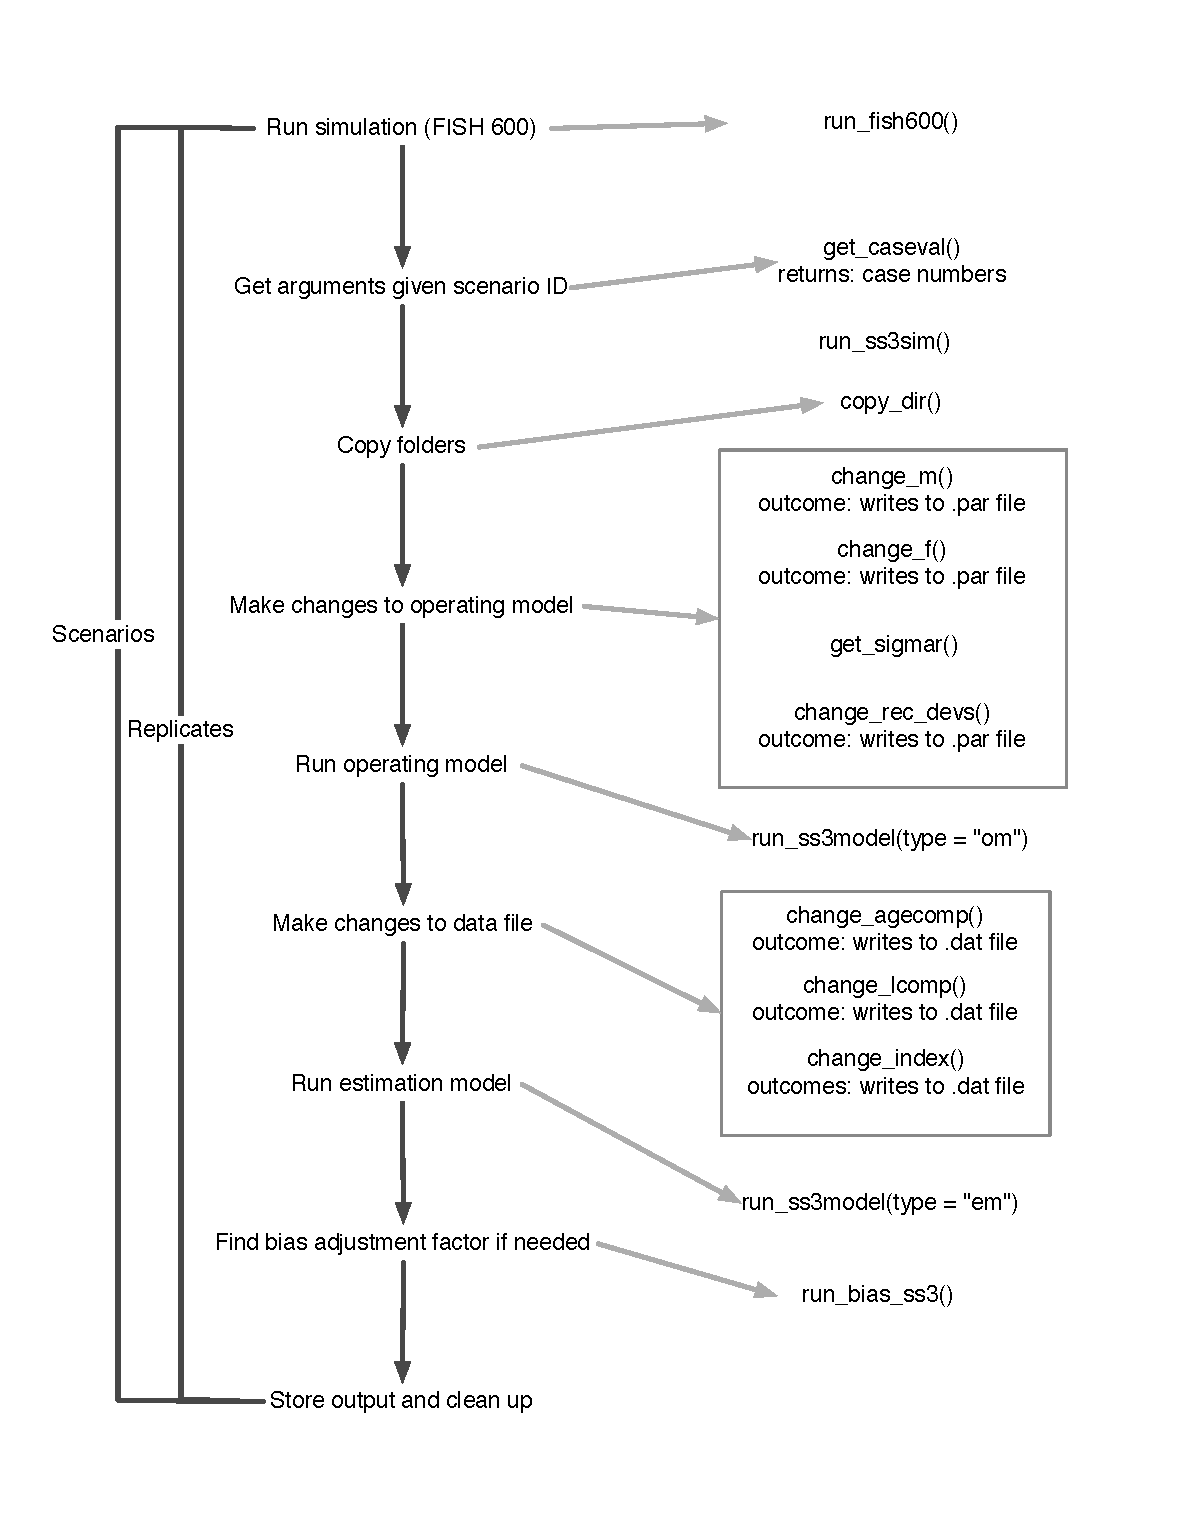
\includegraphics[width=5.5in]{sim-steps.pdf}
  \caption{Simulation steps}
  \label{fig:sim-steps}
\end{figure}


%\noindent
%These functions are used internally by \texttt{run\_simulations} between running
%the operating and estimation models:

%\begin{description}
  %\item[\texttt{change\_lcomp}] Takes a \texttt{data.SS\_new} file, resamples
    %the length compositions from the expected values, and returns a new file
    %with the new length comp samples. Samples can have dimensions, bins, sample
    %sizes, and distributions which are different than those coming from SS.

  %\item[\texttt{change\_agecomp}] Similar to \texttt{change\_lcomp}
    %but for age composition data.

  %\item[\texttt{jitter\_index}] This function is used to create an index of
    %abundance sampled from the expected available biomass for each fleet: survey
    %1 and survey 2 (which mimics the fishery) and add some lognormal errors
    %around it. 
%\end{description}



%\bibliography{/Users/seananderson/Dropbox/tex/jshort,/Users/seananderson/Dropbox/tex/ref}
\end{document}


